%!TEX root = ../MasterThesis.tex

\chapter{Conclusion and Future Work} % (fold)
\label{cha:conclusion}


\section{Decentralized System}
\label{sec:p2p_decentralized_system}

In the decentralized P2P system architecture each node is equal and keeps their local data ready for analysis if the node is online. If the issuer will have to figure out, whether a transaction is fraudulent or not, she is going to send out various queries to all the available nodes in the P2P cluster asking for certain information that help investigating the case. The other nodes, whose reside on each stakeholder involved, will answering the queries based on the common Schema.org data mapping shown above and send back the results to the issuing bank. The issuer will collect all the results from the various parties and combine them to be able to analyze the issue and come up with a conclusion. The main benefit of this architecture is, that there is no need to duplicate the data from the other stakeholders to the issuing bank. Due to this it can also be a better suited solution if data sharing faces restrictions due to law or regulations. On the other hand this architecture will depend on the nodes being online all the time so the issuer can query for information at any time. So this works only in synchronous communication mode. Additionally there are efforts spread around all the stakeholders to set up and maintain a system for secure data querying functionality, please see Figure~\ref{fig:images_p2p_decentralized}.

\begin{figure}[H]
	\centering
		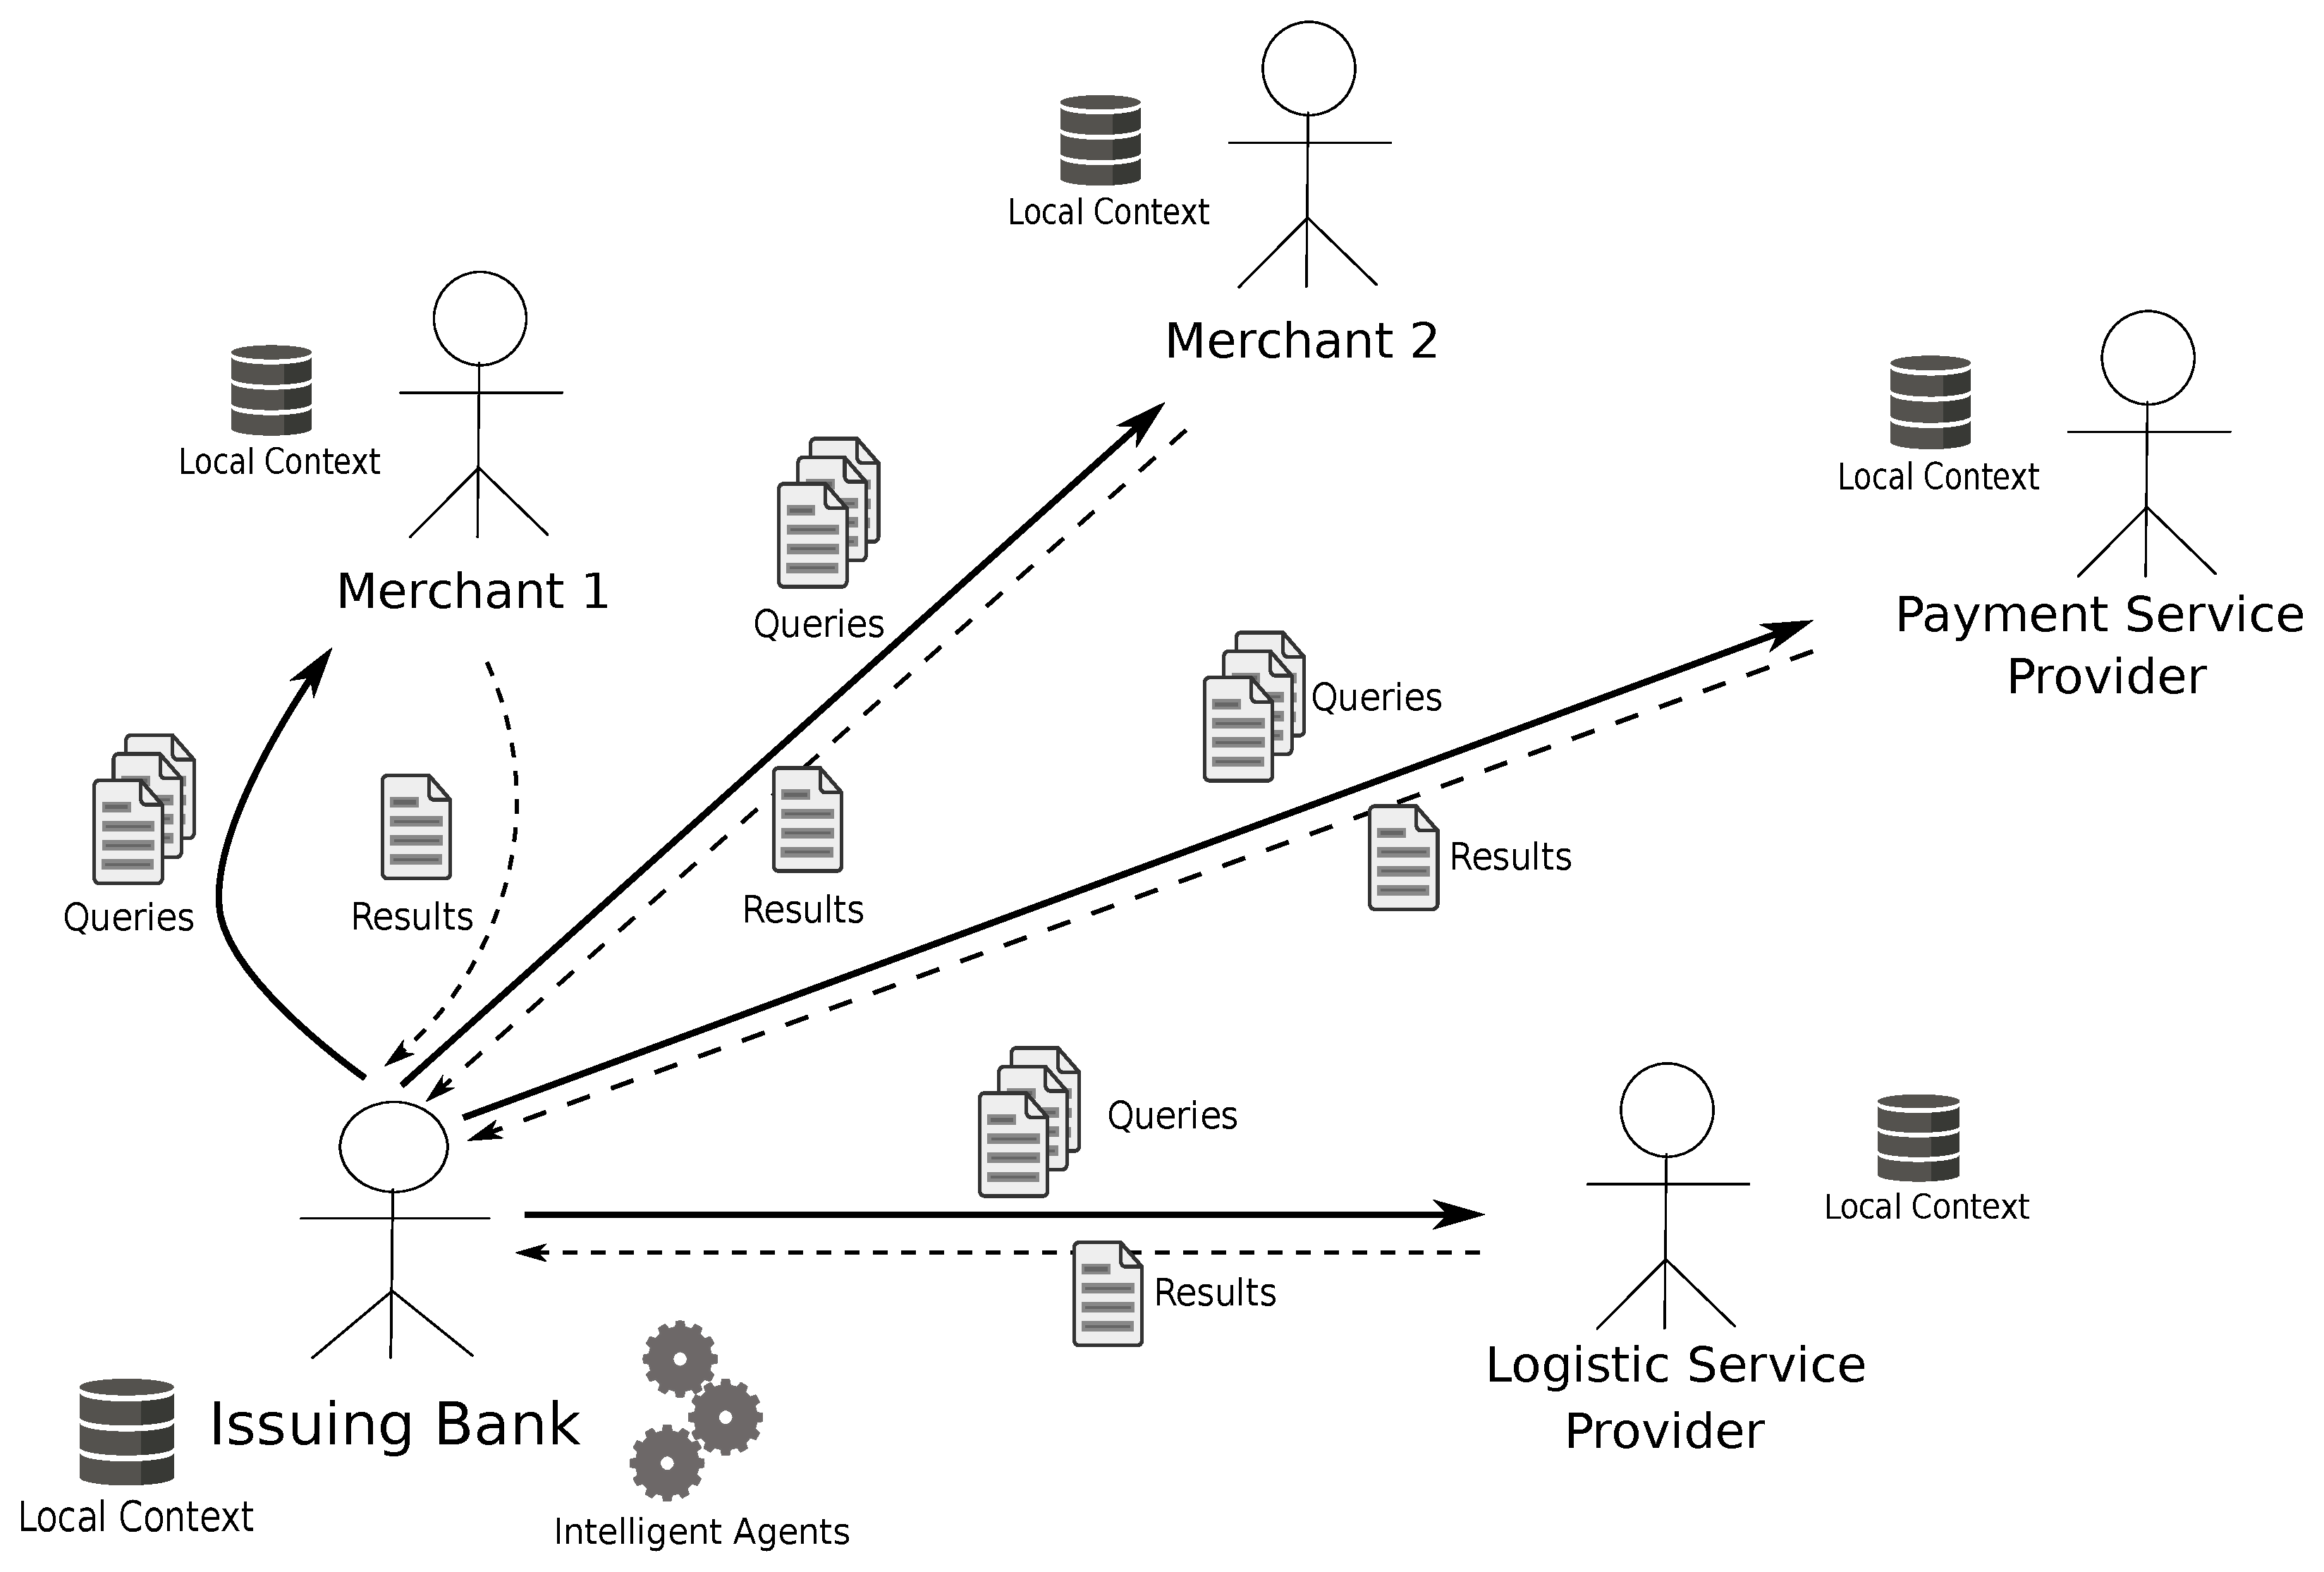
\includegraphics[width=0.8\columnwidth]{images/system_P2P_decentralized.pdf}
	\caption{Decentralized P2P system architecture}
\label{fig:images_p2p_decentralized}
\end{figure}

% sec p2p_decentralized_system

% chapter conclusion (end)
